\documentclass[conference]{IEEEtran}

\usepackage{url}
\usepackage{multirow}
\usepackage{array}
\usepackage{epsfig}
\usepackage{footnote}
\usepackage{amsmath}

\setlength{\parskip}{0pt}
\setlength{\parsep}{0pt}
\setlength{\headsep}{0pt}
\setlength{\topskip}{0pt}
\setlength{\topmargin}{0pt}
\setlength{\topsep}{0pt}
\setlength{\partopsep}{0pt}
\setlength{\floatsep}{0pt}
\setlength{\textfloatsep}{0pt}
\setlength{\intextsep}{5pt}

\widowpenalty=10000
\clubpenalty=10000

\begin{document}

\title{On the Design and Implementation of Autonomic, Decentralized GroupVPNs}

\author{
\IEEEauthorblockA{
  David Isaac Wolinsky$^{\ast}$,
  Linton Abraham$^{\bullet}$,
  Kyungyong Lee$^{\ast}$,
  Yonggang Liu$^{\ast}$,
\\
  Jiangyan Xu$^{\ast}$,
  P. Oscar Boykin$^{\ast}$,
  Renato Figueiredo$^{\ast}$
}
\IEEEauthorblockN{
  $^{\ast}$University of Florida,
  $^{\bullet}$Clemson University
}
}

\maketitle

\begin{abstract}
Virtual private networks (VPNs) enable existing network applications to run
unmodified in insecure and constrained environments by creating an isolated and
secure virtual environment providing all-to-all connectivity for VPN members.
Traditionally VPNs have been used in dedicated systems to connect many users to
a single site or a few sites together through manual configuration.  Recently,
decentralized VPNs have been developed to support those that require systems
with no dedicated resources and reduced configuration overhead.  We extend this
concept to provide a truly novel approach to VPNs, a decentralized,
self-configuring VPN.  To put our approach in prospective, we survey existing
VPN approaches and quantitatively compare a reference implementation of our
approach to existing VPN systems.
\end{abstract}

\section{Introduction}
A Virtual Private Network (VPN) provides the illusion of a local area network
(LAN) spanning a wide area network (WAN) infrastructure by creating encrypted
and authenticated, secure\footnote{For the remainder of this paper, unless
explicitly stated otherwise, security implies encryption and authentication.}
communication links amongst participants.  Common uses of VPNs include secure
access to enterprise network resources from remote/insecure locations,
connecting distributed resources from multiple sites, and establishing virtual
LANs for multiplayer video games over the Internet.  

The architecture described in this paper addresses a usage scenario such as
collaborative academic environments linking individuals spanning multiple
institutions belong to the same virtual organization, where coordinated
configuration of network infrastructure across the different sites is often
impractical.  Another example is the small/medium business (SMB) environment,
where it is often desirable to interconnect desktops and servers across
distributed sites and secure traffic to enterprise networked resources without
incurring the complexity or management costs of traditional VPNs.
Alternatively, consider an academic at a conference who wants their Internet
traffic encrypted to prevent eavesdropping from their peers or desires to
browse websites only available to those on the university network.

In this paper, we discuss an architecture that fits the following requirements:
1) direct communication between remote members, 2) NAT and firewall traversal
or handling, 3) security based on a public key infrastructure (PKI), 4)
decentralized discovery of members in the system, 5) ability to route Internet
traffic through a secure location (full tunnel VPN), 6) self-configuring links
amongst peers, and 7) user interfaces for managing the VPN.

Centralized approaches (e.g.  OpenVPN~\cite{openvpn}) by their very nature
require dedicated infrastructures and do not allow direct communication between
peers though are the only VPN approach to full tunnel operation and guarantee
all-to-all communication regardless NAT and firewall conditions.  P2P-based
approaches (e.g. Hamachi~\cite{hamachi}, Wippien~\cite{wippien},
Gbridge~\cite{gbridge}, PVC~\cite{pvc}) are vulnerable to man-in-the-middle
attacks if session management is handled by an external provider, rely on a
central resource for the creation of VPN links, and require centralized relays
if direct peer communication across NATs and firewalls fails.  Decentralized
approaches require manual configuration of links between members of the virtual
network (e.g., ViNe~\cite{vine}, Violin~\cite{violin}, VNET~\cite{vnet},
tinc~\cite{tinc}).  Existing P2P approaches lack scalability (N2N~\cite{n2n}
and P2PVPN~\cite{p2pvpn}) or are difficult to configure and lack privacy
(I3~\cite{i3}).

To address these issues and meet our requirements, we propose the use of
structured peer-to-peer (P2P) overlay as the fundamental building block to
create a decentralized, dynamic VPN.  We have built a virtual, though not
private, network in previous work~\cite{sc09, ipop}.  In this paper, we consider
the security implications of using a structured overlay and present methods that
create a VPN on top of a structured overlay.  The foundation of our VPN is an
extension of our previous work in~\cite{icdcs10}, where we implemented PKI
secured overlays configured through a Web 2.0 Group infrastructure, to support
the configuration of GroupVPNs.  The other components missing from previous and
related research and work is the lack of decentralized, autonomic creation of
relays and support for full tunnel VPN mode in a decentralized system, our
novel contributions for this paper.  This paper stands alone as a canonical
resource to provide necessary documentation to create a structured P2P VPN
supporting all the requirements listed earlier.

The rest of this paper is organized as follows.  Section~\ref{vpns} discusses
the different VPN approaches including ours which is based upon structured
P2P overlays.  We present our novel contributions of decentralized relays,
full tunnel VPN modes for P2P VPNs, and user-friendly configuration of VPNs
in Section~\ref{relays}, Section~\ref{full_tunnel}, and Section~\ref{groups},
respectively.  To validate the P2P approach, we compare it against centralized
VPNs in Section~\ref{evaluation}.  Finally, we conclude our paper in
Section~\ref{conclusions} with a discussion on real systems using our approach.

\section{Virtual Private Networks}
\label{vpns}
Common VPN architectures are presented in Table~\ref{tab:vpn_types}.  This
section begins by reviewing the fundamental features found in all VPN clients
and then differentiating the components as they relate to the various VPN
approaches, these components include client address allocation, peer discovery
and authentication, and the available security models using real VPN systems.

\begin{table}[ht]
\caption{VPN Classifications}
\label{tab:vpn_types}
\begin{center}
\begin{tabular}[c]{|m{2cm}|m{5.75cm}|} \hline
Type & Description \\ \hline
Centralized & Clients communicate through one or more servers which are statically
configured \\ \hline
Centralized Servers / P2P Clients & Servers provide authentication, session management, and
optionally relay traffic; peers may communicate directly with each
other via P2P links if NAT traversal succeeds\\ \hline
Decentralized Servers and Clients & No distinction between clients and servers;
each member in the system authenticates directly with each other; links between
members must be explicitly defined \\ \hline
Unstructured P2P & No distinction between clients and servers; members either know
the entire network or use broadcast to discover routes between each other \\ \hline
Structured P2P & No distinction between clients and servers; members are usually
within $O(\log N)$ hops of each other via a greedy routing algorithm; use 
distributed data store for discovery \\ \hline
\end{tabular}
\end{center}
\end{table}

\subsection{The Basic Client VPN Configuration}
Figure~\ref{fig:vpn} presents an abstraction of the common features found in
all VPN client, a service that communicates with the VPN system and a virtual
network (VN) device for host integration.  During initialization, the VPN
services authenticates with the overlay~\footnote{An overlay in this context
refers any portion of the VPN system including a central server, another VPN
client, or a relay.}, optionally, querying for information about the network,
such as network address space, address allocations, and domain name service
(DNS) servers.  At which point, the VPN enables secure communication amongst
participants.

There are many ways in which a client authenticates with the overlay.  A system
can be setup quickly by using no authentication or a shared secret such as a key
or a password.  Using accounts and passwords with or without a shared secret
provides individualized authentication, allowing an administrator to block all
users if the shared secret is compromised or individual users who act
maliciously.  In the most secure approaches, each client has a unique signed
certificate making brute force attacks very difficults.  The trade-offs in the
approaches come in terms of security, usability, and management.  While the use
of signed certificates provides better security than shared secrets,
certificates require more configuration and maintenance.  In a system comprising
of non-experts, the usual setup uses a shared secret and individual user
accounts.  The secret is packaged with the VPN application, which is distributed
through secure channels such as authenticated HTTPS.

A VN device allows applications to communicate transparently over the VPN.  The
VN device provides mechanisms for injecting incoming packets into and retrieving
outgoing packets from the networking stack, enabling the use of common network
APIs such as Berkeley Sockets, thereby allowing existing application to work over
the VPN without modification.  While there are many different types of VN
devices, we focus on TAP~\cite{tap} due to its open source and pervasive nature.
TAP allows the creation of one or more Virtual Ethernet and / or IP devices and
is available for almost all modern operating systems including Windows, Linux,
Mac OS/X, BSD, and Solaris.  A TAP device presents itself as a character device
providing read and write operations.  Incoming packets from the VPN are written
to the TAP device and the networking stack in the OS delivers the packet to the
appropriate socket.  Outgoing packets from local sockets are read from the TAP
device.

VN devices can be configured manually though command-line tools or OS' APIs or
dynamically by the universally supported dynamic host configuration process
(DHCP)~\cite{dhcp0}.  Upon the VN device obtaining an IP address, the system
adds a new rule to the routing table that directs all packets sent to the VPN
address space to be directed to the VN device.  Packets read from the the TAP
device are encrypted and sent to the overlay via the VPN client.  The overlay
delivers the packet to another client or a server with a VN stack enabled.
Received packets are decrypted, verified for authenticity, and then written to
the VN device.  In most cases, the IP layer header remains unchanged, while
VPN configuration determines how the Ethernet header is handled.


\begin{figure}[ht]
\centering
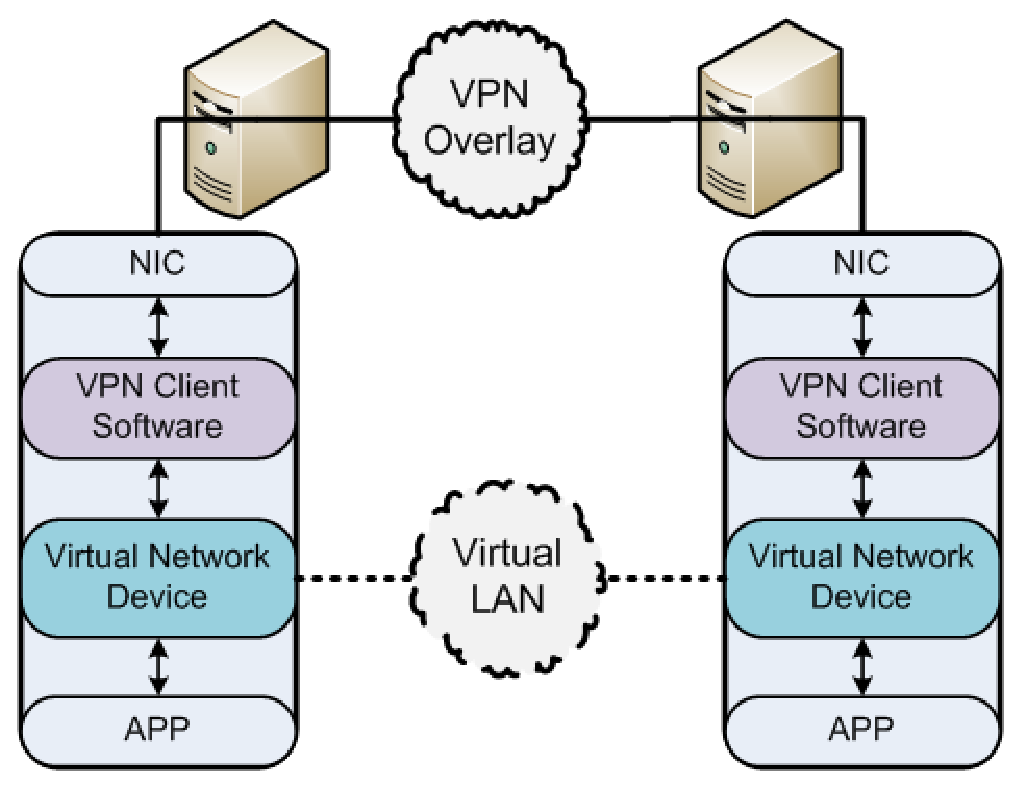
\epsfig{file=figs/vpn.png.eps, width=2.5in}
\caption{A typical VPN client.  A VN device makes application interaction with
the VPN transparent.  Packets going to the VPN destination are sent by routing
rules to the VN device interfaced by the VPN client.  The VPN client sends
and receives packets from other VPN participants via the hosts physical network
device.}
\label{fig:vpn}
\end{figure}

\subsection{Centralized VPN Systems}
OpenVPN is an open and well-documented platform for deploying centralized VPNs.
We use it as the basis for understanding centralized VPNs as it represents
features common to most centralized VPNs.  In centralized VPN systems, clients
forward all VPN related packets to the server.  Clients responsibilities are
limited to configuring the VN device and authenticating with the VPN server;
whereas the servers are responsible for authentication and routing between
clients and providing access to the servers' local resources and the Internet
(full tunnel).

While central VPNs do support multiple servers, the client must know of all
existing servers randomly selects a server, implementing a simple load
balance.  Once connected, servers hand to the client an IP address in the
VPN address space.  Depending on configuration this will allow a client to
communicate with other clients, resources on the same network as the server,
or Internet hosts via the VPN.  Additionally, servers must be configured to
connect with all other servers otherwise clients behind remote servers will
not be able to communicate with each other.

All inter-client communication flows through the central server.  By default, a
client encrypts a packet and sends it to the server.  Upon receiving the packet,
the server decrypts it, determines where to relay it, encrypts it, and then
sends the packet to its destination.  This model allows a server to eavesdrop on
communication.  While a second layer of encryption is possible through a shared
secret, it requires out-of-band communication and increases the computing
overhead on communication.

\subsection{Centralized P2P VPN Systems}
Hamachi~\cite{hamachi} is the first well known centralized VPN that used the
ambiguous moniker ``P2P VPN''.  In reality, these systems would be best
classified as centralized VPN servers with P2P clients.  Other similar VPNs
include Wippien~\cite{wippien}, Gbridge~\cite{gbridge}, and PVC~\cite{pvc}.
Specifically, P2P in these systems is limited to direct connectivity between
clients orchestrated through a central server.  In the case where direct
connectivity is unavailable due to NATs or firewalls, the central server can
act as a relay and if not peers will be unable to communicate.  Each approach
uses their own security protocols that involve using a server to verify the
authenticity and setup secure connections between clients.  Furthermore, most
of these projects are closed preventing users from hosting their own
authentication servers and relays and verifying the code for security purposes
forcing users to trust the third-party server to not eavesdrop or perform other
man-in-the-middle attacks.

\subsection{Decentralized VPN Systems}
Some examples of systems that assist in distributing load in VPN systems are
tinc~\cite{tinc}, CloudVPN~\cite{cloudvpn}, ViNe~\cite{vine}, VNET~\cite{vnet},
and Violin~\cite{violin}.  These systems are not autonomic and require explicit
specification of links between resources.  This means that, like OpenVPN, these
systems can suffer VPN outages when nodes go offline, thus administrators must
maintain the VPN connection table.  Unlike OpenVPN, these approaches typically
do not require all-to-all direct connectivity for all-to-all communication.
Users can either setup out-of-band NAT traversal or route through relays.  Users
must manually create links with those whom they desire maximum network
performance.

\subsection{Unstructured P2P VPN Systems}
Unlike centralized and decentralized systems, P2P environments are
self-configuring requiring the only task for the user is to connect to the
P2P overlay.  The most simplest form of overlays are unstructured, where peers
form random connections with each other and use broadcast and stochastic
techniques to find information and other peers, though due to its unstructured
nature, the system cannot guarantee distance and routability between peers.
Two examples of unstructured P2P VPNs are N2N~\cite{n2n} and P2PVPN\footnote{Due
to the similarities between the name P2PVPN and focus of this paper, we use
``P2PVPN'' to refer only to ~\cite{p2pvpn} and ``P2P VPN'' to refer explicitly
to the use of P2P in VPNs.}~\cite{p2pvpn}.  P2PVPN is somewhat of a hybrid
using a centralized BitTorrent tracker to assist in peers finding each other,
they eventually will also be able to search for each other using the overlay.
In N2N, peers first connect to super nodes and then to find another peer they
broadcast discovery messages to the entire overlay.  In the case that peers
cannot form direct connection, peers can route to each other over the N2N
overlay.  While unstructured P2P systems have some scalability concerns, they
provide a server-less approach.  In the realm of VPNs, all client VPNs are also
servers performing authentication though neither approach deals with
decentralized address allocation.

\subsection{Structured P2P VPN Systems}
To address the scalability concerns in unstructured systems, our approach uses
structured P2P overlays.  Structured P2P overlays provide distributed look up
services with guaranteed search time with a lower bound of $O(\log N)$, in
contrast to unstructured systems, which rely on global knowledge/broadcasts, or
stochastic techniques such as random walks~\cite{unstructured_v_structured}.
Some examples of structured systems can be found are Pastry~\cite{pastry},
Chord~\cite{chord}, Symphony~\cite{symphony}, Kademlia~\cite{kademlia},
CAN~\cite{can}, and Brunet~\cite{brunet}.  In general, structured systems are
able to make these guarantees by self-organizing a structured topology, such as
a 2D ring or a hypercube, deterministically by randomly generated node
identifiers.

Most structured P2P overlays support decentralized storage/retrieval of
information by mapping keys to specific node IDs in an overlay called a
distributed hash table (DHT).  At a minimum, the data is stored at the node ID
either smaller or larger to the data's node ID and for fault tolerance the data
can be stored at other nodes.  

Our previous work,\cite{sc09}, describes a virtual, though not private, network
using structured P2P overlays.  This system provides the underying VN component
for the VPN described in this paper.  In this system, each VN has a unique
identifier or namespace so that the VPNs can share a common overlay.
To perform address allocation, peers perform atomic writes into the structured
overlays DHT, where the key is a hash of the VPN's namespace and the desired
address and the value is the peer's node ID.  A successful write implies that
the user was the first to have written a value to that key resulting in a
successfully reserved IP address.  When an IP packet arrives in the system
destined for an unknown host, the VPN queries the overlay's DHT using the hash
of the VPN's namespace and remote peer's IP address.  A successful query will
result in retrieving an overlay ID, the location where the VPN should forward
all IP packets for that VPN IP.  Since packets are initially routed over the
overlay the performance can be undesirably slow, thus after communication has
surpassed a few packets, the peers form direct connections via the overlay.

To provide privacy, a VPN must have secure links between communicating peers.
In free-to-join structured overlays, this will not be enough as the DHT can
easily become polluted or the overlay may become unreliable due to malicious
peers~\cite{sybil}.  There are many works towards tamper resistant overlays,
they do not map well to existing security standards used in VPNs, such as a
PKI or shared secrets.  These approaches limit the availability of the overlay
to trusted users making them no longer free-to-join.  This issue has been
address in our previous work, \cite{icdcs}, which presents a method by which
a public overlay is used to bootstrap a private overlay secured by PKI.  Peers
first join the public overlay, then using the public overlays DHT to find
other peers in the private overlay.  Peers send encrypted and authenticated
connection messages over the public overlay.  The approach allows peers to find
each other using a free-to-join overlay to form their own private overlays
enabling the construction of an overlay constructed of peers behind NATs and
firewalls, who would otherwise be unable to form their own overlay.  In the
private overlay, both IP and overlay control messages are secured using the PKI
encrypted and authenticated using DTLS~\cite{dtls}, thus if a peer misbehaves
in the overlay, they can easily be revoked using both a revocation list or a
broadcast revocation in the overlay~\cite{icdcs}.

I3~\cite{i3} or Internet Indirection Infrastructure provides an alternative
structured overlay approach.  Peers use the DHT similarly to IPOP, though there
is no discussion on address exclusivity.  Unlike IPOP, I3 does not provide
direct communication between peers, but rather, indirect communication so that
peers never discover each others real identities.  The purpose of I3 does not
align with the requirements set forth in the introduction.

\section{Dealing with Oppressive NATs and Firewalls}
\label{relays}
As of 2010, the majority of the Internet is connected via Internet Protocol (IP)
version 4.  A limitation in this protocol is that there are only $2^{32}$
addresses total though or approximately 4 billion addresses.  With the
Earth already having a population of over 8 billion and each individual having
multiple devices that have Internet connectivity the IPv4 limitation is becoming
more and more apparent.  To address this issue there have been two focuses:  1)
the use of network address translation (NAT) to enable many machines and devices
to share a single IP address but preventing bidirectional connection initiation
and 2) IPv6 which supports $2^{128}$ addresses.  IPv6 does not necessarily imply
direct connectivity as there are no guarantees of NAT disappearing and outbound
only firwalls allowing incoming connections.

Approaches for handling NAT and firwall traversal come from two main branches:
hole punching and relaying.  When performing hole punching, peers
simulataneously attempt to create "holes" in their NAT / firewall devices
allowing direct TCP or UDP communication with a peer behind another NAT /
firewall.  This works by confusing the NAT into believing that the peer
behind that NAT initiated the connection.  NATs work by making IP:Port mappings
and so if two peers do this simulataneously, they may be able to have both of
their NATs create these holes allowing direct communication.  TCP NAT hole
punching, though, does not work on systems that use stateful firewalls.
Relaying, on the other hand, always works as peers behind NATs communicate with
a third peer with whom they have have direct connectivity, though with the side
effect of additional latency and the cost for the relay of supporting the
bidirectional communication.

\subsection{Relays}
Centralized and decentralized VPNs do not suffer from this problem as all
traffic passes through the central server or managed links.  In the
unstructured examples, P2PVPN does not support any form of relaying though
N2N allows peers to communicate through the overlay when traversal fails.
Simiarly a structured P2P VPN can use the overlay, though as an overlay
grows in size, so does the hop count between peers increasing latency and
potentially creating a bandwidth bottle neck.  This issue can be addressed
through a distributed, autonomic relaying system.  Building upon previous
work~\cite{hpdc08_0}, wherein, peers next to each other in the overlay's node
ID space communicate ``directly'' through overlapping connections due to
firewall, NAT, or Internet fragmentation issues.  

When two nodes discover each other via the overlay and attempt to become
connected but fail during NAT and firewall traversal, they exchange peer
lists through the overlay.  Upon receiving this list, the two peers identify
the overlap in the neighbor sets to form a two-hop connection.  When peers
are not located near each other in the overlay, most likely they will have
no overlap.  This can be addressed by having peers connect to each other's
neighbor set proactively creating overlap, as represented in
Figure~\ref{fig:relay}.

\begin{figure}[ht]
\centering
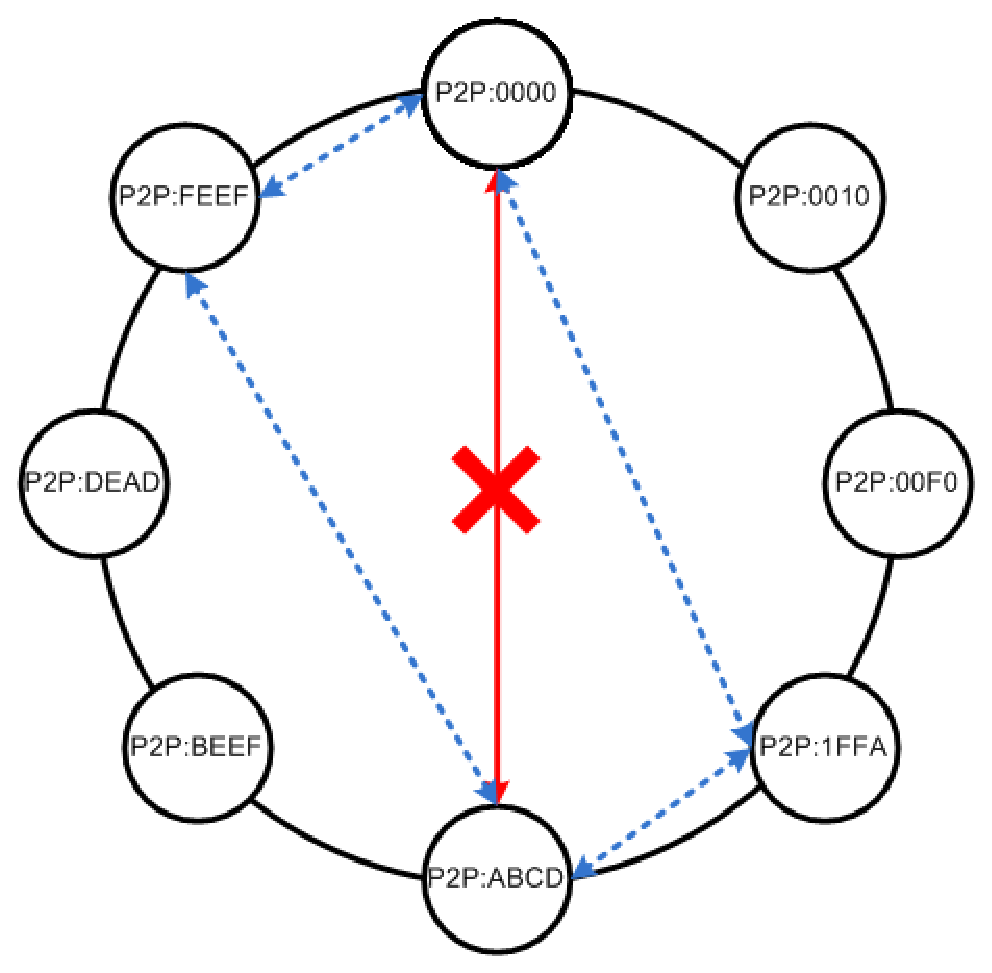
\epsfig{file=figs/relay.png.eps, width=2.75in}
\caption{Creating relays across the node address space, when direct
connectivity is not possible.  Two members, 0000 and ABCD,  desire a direct
connection but are unable to directly connect, perhaps due to NATs or firewalls.
They exchange neighbor information through the overlay and connect to one of
each other's neighbors, creating an overlap.  The overlap then becomes a 
relay path (represented by dashed lines), improving performance over routing
across the entire overlay.}
\label{fig:relay}
\end{figure}

In addition to exchanging overlap, peers also exchange some state of their
connections with the neighbors.  For example, the data shared could be
regarding node stability as measured by the age of a connection and proximity
as measured by ping latency to the neighbor.  When creating overlap or overlap
changes, peers review these metrics to decide which subset of the overlap to
use as a proxy leaving the remaining peers as reserves.

\subsection{Usefulness of Relays}
To verify the usefulness of two-hop over overlay routing, we have evaluted
the latency approach using an event-driven simulator that reuses the code
base of IPOP to faithfully implement its functionality using event-driven
simulated times to emulate WAN latencies.  For this experiment, we chose
latencies based upon the MIT King Data Set~\cite{king_data}, which consists of
all-to-all latencies between 1,740 well-distributed Internet hosts.  We
then evaluated overlays using various network sizes up to 1,740.  After
starting the overlay, we wait for it to reach steady state, when the overlay
is completely formed and no new connections are created, then we calculate
the average all-to-all latency for all messages that would have taken two
overlay hops or more, the average of our low latency relay model, and the
average of single hop communication.  In the low latency relay model, each
destination node form a connection to the source node's physically closest peer
as determined via latency (in a live system by application level ping).  Then
this pathway is used as a two-hop relay between source and node.  We only look
at two overlay hops and more, as a single hop would only benefit under
triangular inequalities that are not a consideration in our work.  The
simulations were performed on a distributed grid platform, Archer~\cite{archer},
that uses IPOP for its virtual networking component. 

\begin{figure}[ht]
\centering
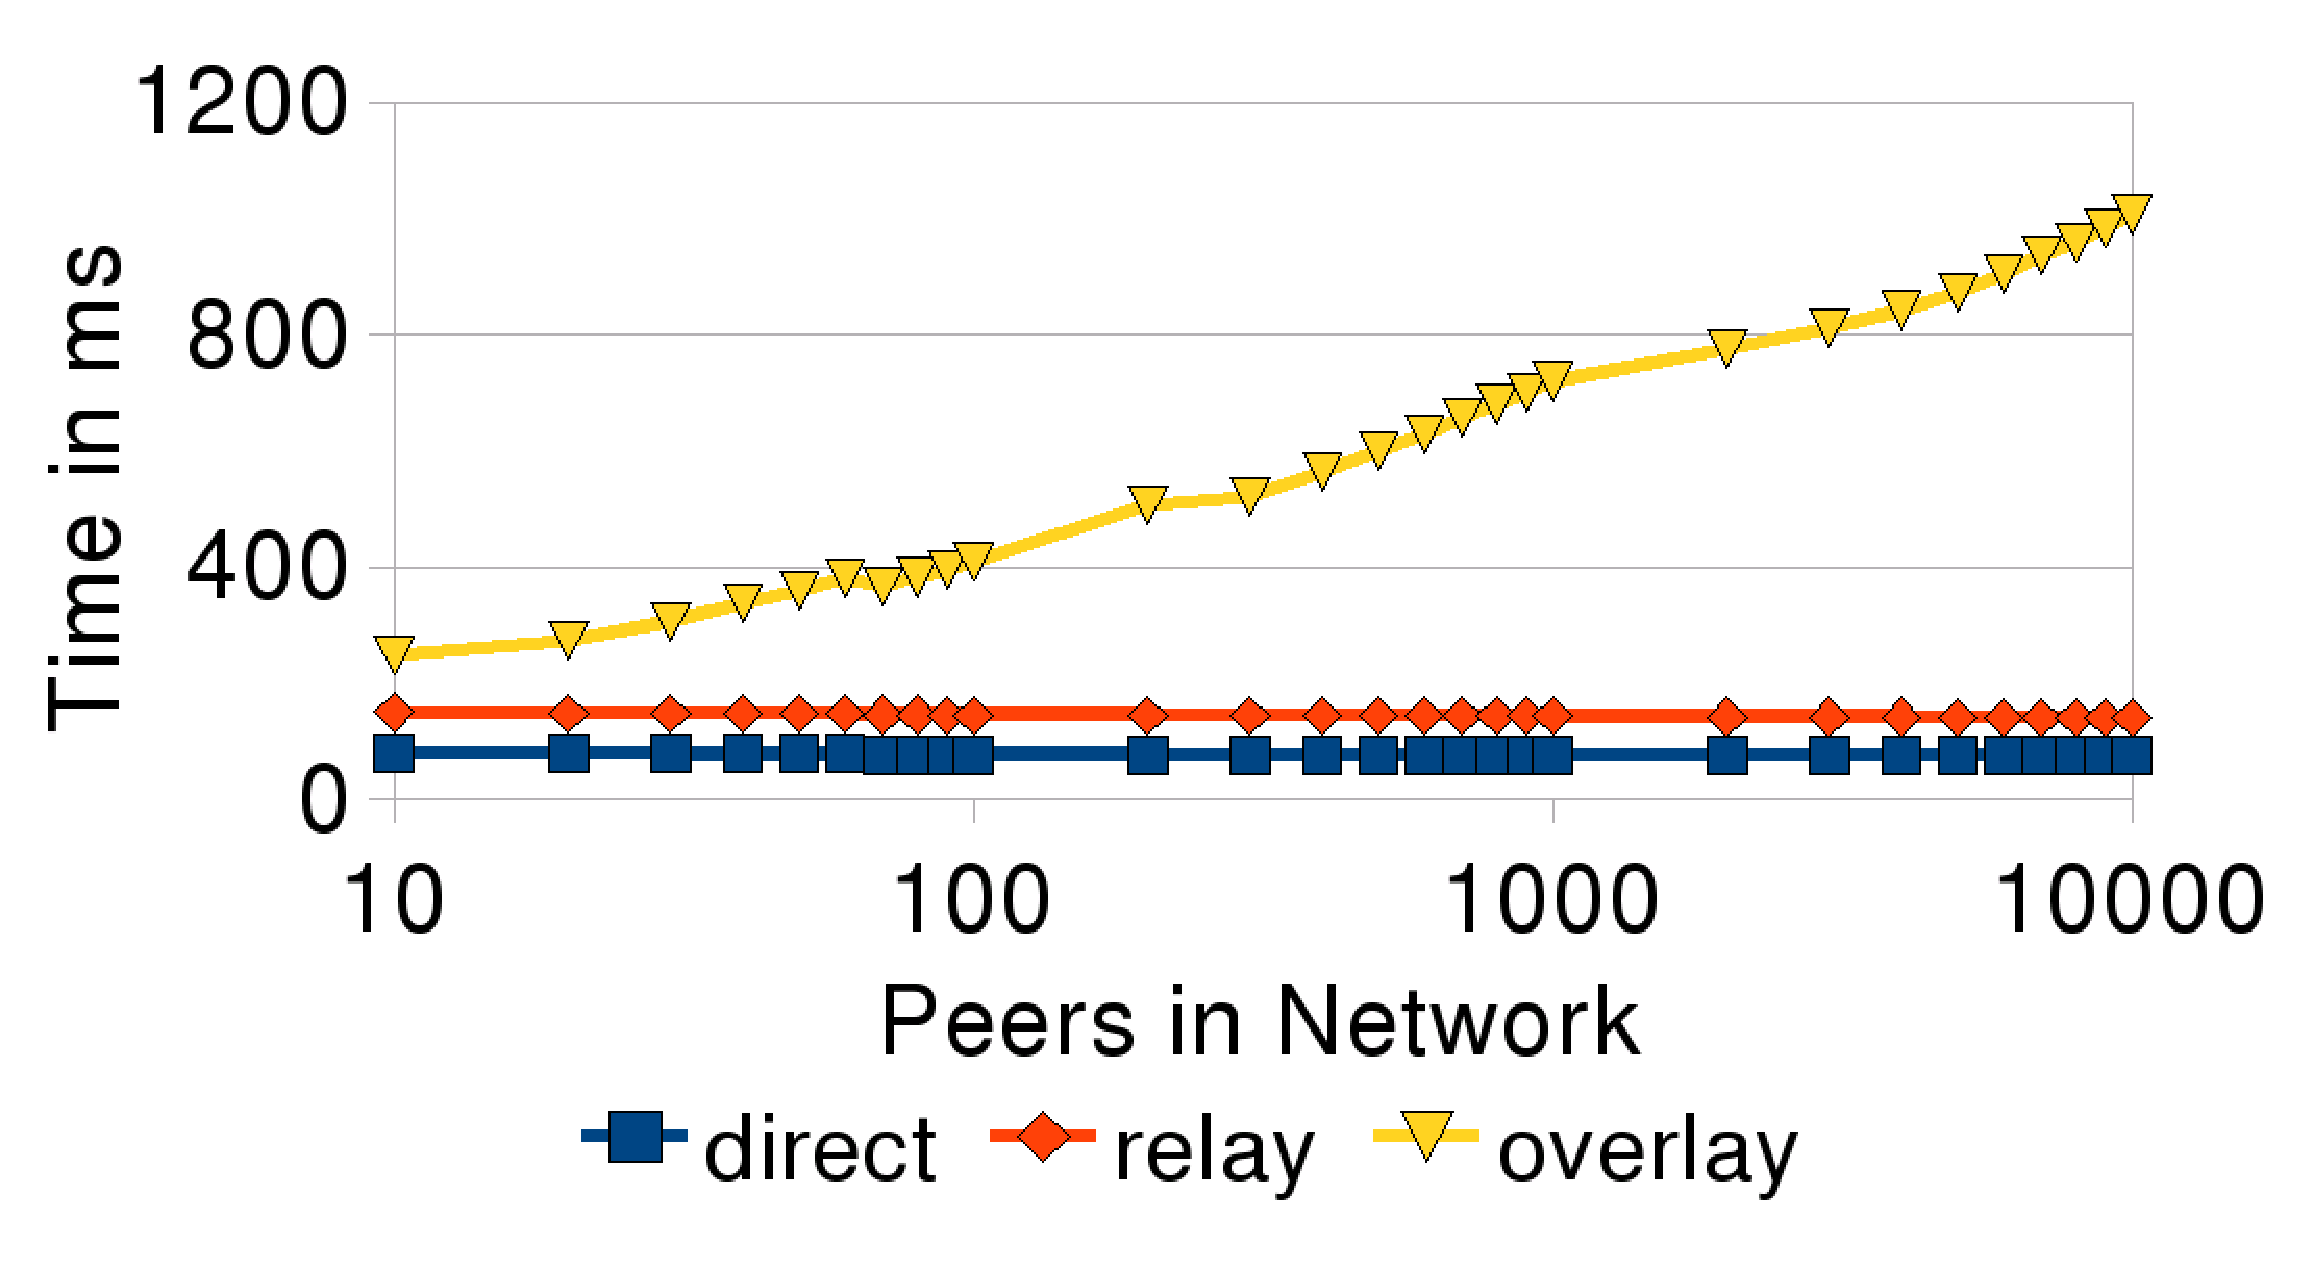
\epsfig{file=figs/relay_motivation.png.eps, width=3in}
\caption{A comparison of the average all-to-all overlay routing, two-hop relay, and
direct connection latency in a Structured P2P environment, Brunet, using the King
data set.}
\label{fig:simulated_relays}
\end{figure}

Our results are presented in Figure~\ref{fig:simulated_relays}.  We performed
the tests for varying network sizes.  We began our tests at 25, because network
sizes around 20 and under tend to be fully connected due to the connectivity
requirements of the system.  It is not until the network size expands past 100
and towards 200 nodes that relays become significantly beneficial.  At
100 nodes, there is approximately a 54\% performance increase, whereas at
200 there is an 87\% increase and it appears to grow proportionately to the size
of the pool.  The key take away is that latency-bound applications
using a reasonably sized overlay would significantly benefit from
the use of two-hop relays.  

Additionally, we verified their use in a reference implementation of our VPN
using a real system.  The environment consists of using PlanetLab as the public
overlay and our Archer environment as the VPN environment.
PlanetLab~\cite{planetlab} provides a set of over 500 distributed computing
nodes all with public IP addresses.  Archer provides grid computing to computer
architecture researchers and consists of over 500 nodes located at various
academic sites.  To ensure that peers formed two-hop connections, we instituted
a firewall preventing direct communication between the two.  In tests, we found
that the peers were always able to find a good relays, the bandwidth and latency
averages were 2245 Kbit/s $\pm$ 1080 and 58.1 ms $\pm$ 35.5, respectively.

\section{Full Tunnel VPN Operations}
\label{full_tunnel}
The configuration detailed so far describes a split tunnel: a VPN connection
that handles \emph{internal VPN traffic only and not Internet traffic}.  Prior
to this work, only centralized VPNs currently support full tunnel: a VPN that
provides the features of a split tunnel in addition to securely forwarding
\emph{all their Internet traffic} through a VPN gateway.  A full tunnel provides
network-layer privacy when a user is in a remote, insecure location such as an
open wireless network at a coffee shop by securly relaying all Internet traffic
through a trusted third party, the VPN gateway.  Both models are illustrated
in Figure~\ref{fig:tunnel}.

\begin{figure}[ht]
\centering
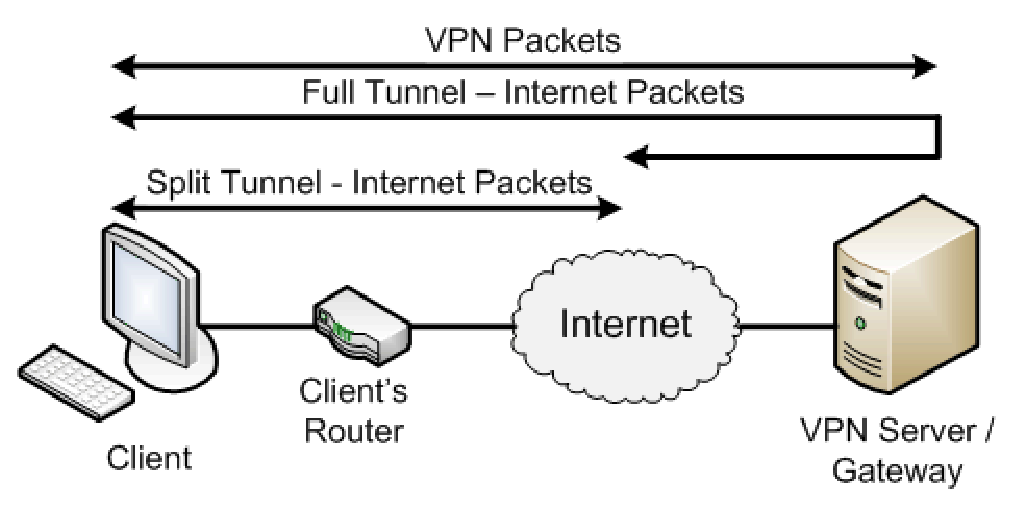
\epsfig{file=figs/tunnel.png.eps, width=2.75in}
\caption{An example of both full and split tunnel VPN modes.  In both, packets
for the server are sent directly to the server.  In split tunnel mode, Internet
packets bypass the VPN and are routed directly to the Internet.  In full tunnel
mode, Internet packets are first routed to the VPN gateway, and then to their
Internet destination.}
\label{fig:tunnel}
\end{figure}

Central VPN clients use full tunneling through a routing rule swap, setting
the default gateway to be an endpoint in the VPN subnet and traffic for thE
VPN server is routed explicitly to the LAN gateway.  This rule swap causes
all Internet packets to be routed to the VN device and the VPN software
can then send them to the remote VPN gateway.  At the VPN gateway, the packet
is decrypted and delivered to the Internet.  A P2P system encounters two
challenges in supporting full tunnels:  1) P2P traffic must not be routed
to the VPN gateway and 2) there may be more than one VPN gateway.  We address
these issues and provide a solution to this problem in Section~\ref{full_tunnel}.

The challenges we face in our VPN are providing decentralized discovery of a
VPN gateway and supporting full tunnel mode in a P2P environment such that
all P2P traffic is sent to the intended receiver directly instead of through
the gateway.  The remainder of this section covers our gateway and client
solutions to address these challenges.

\subsection{The Gateway}
\label{the_gateway}
A gateway can be configured through NAT software, like masquerading in IPtables
or Internet Connection Sharing with Windows.  This automatically handles the
forwarding of packets received on the NAT interface to another interface
bringing the packet closer to its destination.  Similarly, incoming packets
on the outgoing interface must be parsed in order to determine the destination
NAT client.

Following from our previous work on VPNs~\cite{sc09}, if a VPN is a gateway,
the VPN state machine no longer rejects packets, when the destination is not
in the VPN subnet, though when the VPN gateway mode is disabled these packets
are still rejected.  When enabled, all Internet and non-VPN based traffic is
written to the TAP device setting the destination Ethernet address to the TAP
device.  The remaining configuration is identical to other members of the
system as packets from the Internet will automatically have the clients IP as
the destination as a product of the NAT.  To provide for dynamic,
self-configuring systems, VPN gateways announce their availability via an entry
in the DHT.  As future work, this approach can be explored to provide
intelligent selection and load balancing of gateways.

\subsection{The Client}
VPN Clients wishing to use full tunnel must redirect their default traffic to
their VN device.  In our VPN model, we use a virtual IP address for the purpose
of providing distributed VN services DHCP and DNS.  This same address is used
as the the default gateway's IP.  Because this IP address never appears in a
Internet bound packet, only its Ethernet addres does, as shown in
Figure~\ref{fig:tunnel_packet}, this approach enables the use of any and
multiple remote gateways.

To support full tunnel mode, the VPN's state machine has to be slightly modified
to handle outgoing packets destined for IP addresses outside of the VPN, only
rejecting them when full tunnel client mode is disabled.  When enabled, the VPN
software sends packets to the remote peer acting as a full tunnel gateway.
Likewise, incoming packets that have a source address outside the subnet should
not be rejected but instead the overlay address should be a certified VPN
gateway prior to forwarding the packet.

\begin{figure}[ht]
\centering
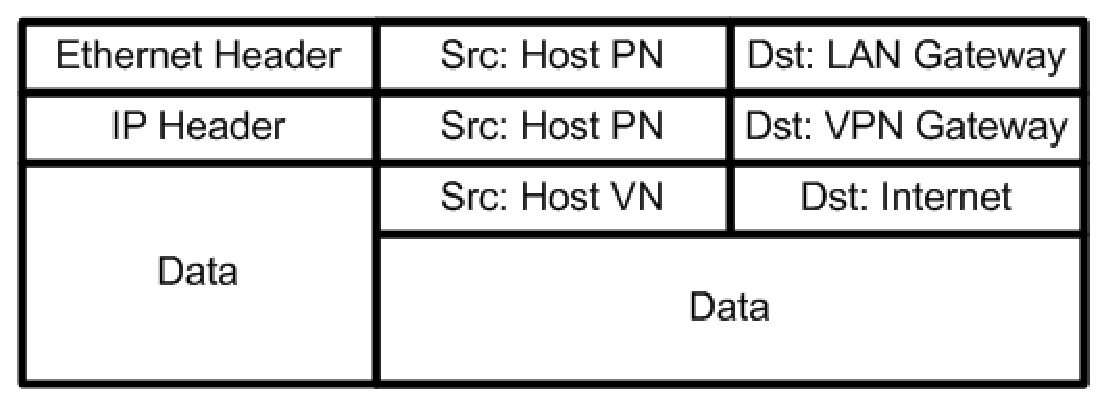
\epsfig{file=figs/tunnel_packet.png.eps, width=2.75in}
\caption{The contents of a full tunnel Ethernet packet.  PN and VN are defined
as physical and virtual network, respectively.}
\label{fig:tunnel_packet}
\end{figure}

To select a remote gateway, peers query the DHT.  As there may be multiple
gateways in the system, the peer randomly selects one, forwarding packets to
that node.  To ensure reliability, when the client has not heard from the
gateway recently, the client sends a liveness query to the gateway.  If the
gateway is down, we take a pessimistic approach and find a new gateway when
the next Internet packet arrives.

The real challenge in applying full tunnel VPN mode to P2P VPNs is the nature
of the P2P system, namely dynamic connections.  Peers do not know ahead of time
what remote peer connections will be thus a simple rule switch does not work.
Our original thought was to watch incoming connection requests and adding
additional routing rules on demand, though this is only reasonably feasible
with UDP as a TCP handshake message would need to be intercepted and potentially
replayed by the local host in order to enable the rule and allow proper routing.
The real drawback of the approach though is that UDP messages can easily be
spoofed by remote peers enabling unsecured Internet packets to be leaked in the
public environment.  Even if the connections are secured, it could take some
time for the peers to recognize a false connection attempt and delete the rule.

To solve the security problem, we propose an alternative, have all traffic
directly routed to the VN device with no additional routing rules.  The VN is
then responsible for filtering P2P traffic and forwarding it to the LAN's
gateway via Ethernet packets.  In the VPN application, outgoing IP packets'
source ports are compared to VPN application's source ports.  Upon a match,
the VPN application directs the packet to the LAN's gateway.  The three steps
involved in this process are 1) translating the source IP address to match the
physical Ethernet's IP address, 2) encapsulating the IP packet in an Ethernet
packet with a randomly source address~\cite{sc09} and the destination the
LAN's gateway, and 3) sending the packet via the physical Ethernet device.
Sending an Ethernet packet is not trivial as Windows lacks support for this
operation and most Unix systems require administrator privilege.  Our platform
independent solution uses a second TAP device bridged to the physical Ethernet
device, allowing Ethernet packets to be sent indirectly through the Ethernet
device via the TAP device.  Because our solution results in incoming packets to
arrive at a different IP address than the actual original source IP address TCP
does not work in this solution.  This method has been verified to work on both
Linux and Windows using OS dependent TAP devices and bridge utilities.

\subsection{Full Tunnel Overhead}
\label{full_tunnel_eval}
While our full tunnel client method effectively resolves the lingering problem
of ensuring that all packets in a full tunnel will be secure, it raises an
issue:  could the effect of having all packets traverse the VPN application be
prohibitively expensive.  To analyze this, we have implemented our approach
and compared it to one that uses the routing rule switch.  In
Figure~\ref{tab:full_tunnel_eval}, we present the ping time from a residential
location to one of Google's IP addresses using a gateway located at the
University of Florida when the VPN is in split tunnel mode, full tunnel using
the routing rule switch, and full tunnel using Ethernet forwarding.  The
results express that there is negligible difference between the full tunnel
approaches.  One interesting result is the latency to gateways public address
in the routing test, which most likely is a result of the ping being sent
insecurely avoiding the VPN stack completely.

\begin{figure}[ht]
\begin{center}
\begin{tabular}[c]{|m{1.5cm}||m{1.25cm}|m{1.25cm}|m{1.25cm}|} \hline
& Google & GW Pri & GW Pub \\ \hline \hline
Ethernet & 70.6 & 12.9 & 13.9 \\ \hline
Routing & 71.4 & 13.2 & 11.0 \\ \hline
None & 66.1 & N/A & 10.9 \\ \hline
\end{tabular}
\end{center}
\label{tab:full_tunnel_eval}
\caption{Latency results comparing full tunnel approaches measured in ms.
Legend: GW Pri - gateway's VPN address, GW Pub - gateway's VPN address,
Ethernet - full tunnel Ethernet packet method, Routing - full tunnel routing
rule switch, None - split tunnel or no VPN.}
\end{figure}

\section{Enabling User-Friendly VPN Operation Through Groups}
\label{groups}
A Group based Web 2.0 environment enables collaborative environments in a
user-friendly approach.  The roles in a group environment are users who can
join and create groups and administrators who can accept or deny join requests,
remove users, and promote other users to administrators.  To apply this to a
VPN\footnote{Note: this is an extension of the group work we have done for
overlays as presented in~\cite{icdcs10}, the entire environment is not novel,
but the application to VPN is}, we consider the group environment as a wrapper
around a public key infrastructure (PKI), where the administrators of the group
act as the certificate authority (CA) and the members have the ability to
obtain signed certificates.  Elaborating further, when a user joins a group,
the administrator can enable automatic signing of certificates or require prior
review; and when peers have overstayed their welcome, they can have their
certificates revoked by removing them from the group.  As described
in~\cite{icdcs10}, revocation can be stored as a CRL on the group site or
distributed through broadcast and DHT on the overlay.  Though we argue for the
use of a user revocation list URL as opposed to a CRL, as a URL can easily
handle cases where a malicious user has automatically signed large amounts of
certificates.

During the creation of the group, the administrator configures the VPNs address
range, namespace, enabling security, and if they would like to use an existing
overlay network or provide their own set of overlay nodes.  When a user has
been accepted into the group, they are able to download VPN configuration data,
that assists in the self-configuration of the VPN.  The configuration is
self-contained and requries that the user provide it to the VPN, by either
placing it in a specific directory, a GUI, or a command-line utility whose only
input parameter is the path to a configuration file.  Though in our system, we
have only implemented the file system and command-line approaches.  The
configuration data contains the IP address space, VPN namespace, group website's
address, and a shared secret.  The shared secret uniquely identifies the user,
so that the website can determine how to handle certificate requests.  When
making a certificate request, the user sends over HTTPS a public key and their
shared secret, the website creates and signs a certificate request based upon
the public key and the user's relevant information ensuring that users cannot
trick the website into signing malicious data.  Upon receiving the signed
certificate, peers are able to join the private overlay and VPN enabling
secure communication amongst the VPN peers.

\section{Evaluation of VPN Models}
\label{evaluation}
This experiments explores bandwidth and latency in a distributed VPN system to
motivate the usage of P2P links in a VPN.  The VPNs used are our reference
implementation (IPOP), OpenVPN, and Hamachi.  OpenVPN represents a typical
centralized VPN, while Hamachi represents a well-tuned P2P-link VPN.  The
evaluation was performed on Amazon EC2 using small instance sized
Ubuntu i386 instances to create various sized networks ranging from 1 to 32.
OpenVPN uses an additional node as the central server and Hamachi has an upper
bound of 16 due to limitations in the Linux version at the time of this
evaluation.  To perform bandwidth tests, the instances are booted and query an
NFS for the list virtual IP addresses, peers are ordered such that half the
peers are act as clients and the other half the peers creating a 1 to 1 mapping
between all sets.  Latency and bandwidth tests are performed using netperf's
request-reply and streaming tests respectively.  Prior to the start of the
tests, peers have no knowledge of each other, except the virtual IP addresses,
thus connection startup costs are included in the test.  Test are run for 10
minutes diluting the connection initiation overhead but represent an example of
real usage.  Results from the clients are polled at all locations and averaged
together, though the OpenVPN server is measured separately.  IPOP and OpenVPN
use authenticated 128-bit AES, while Hamachi does not allow configuration of
the security parameters and uses the default Hamachi settings.

\begin{figure}[ht]
\centering
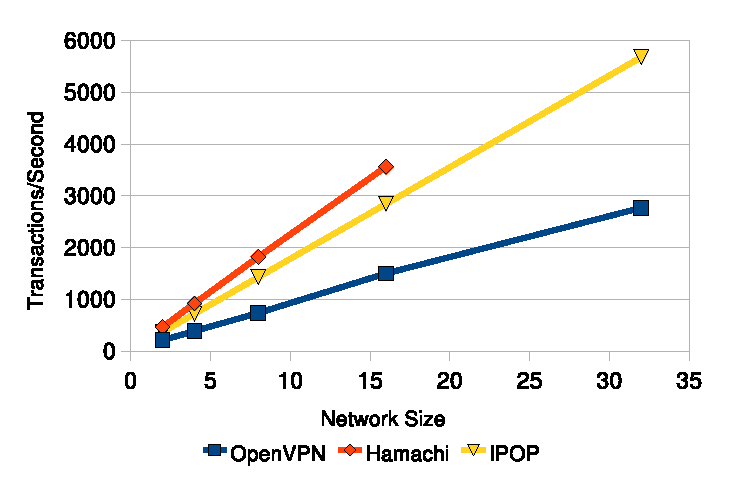
\epsfig{file=figs/latency.eps, width=3in}
\caption{System transaction rate for various VPN approaches.}
\label{fig:latency}
\end{figure}

\begin{figure}[ht]
\centering
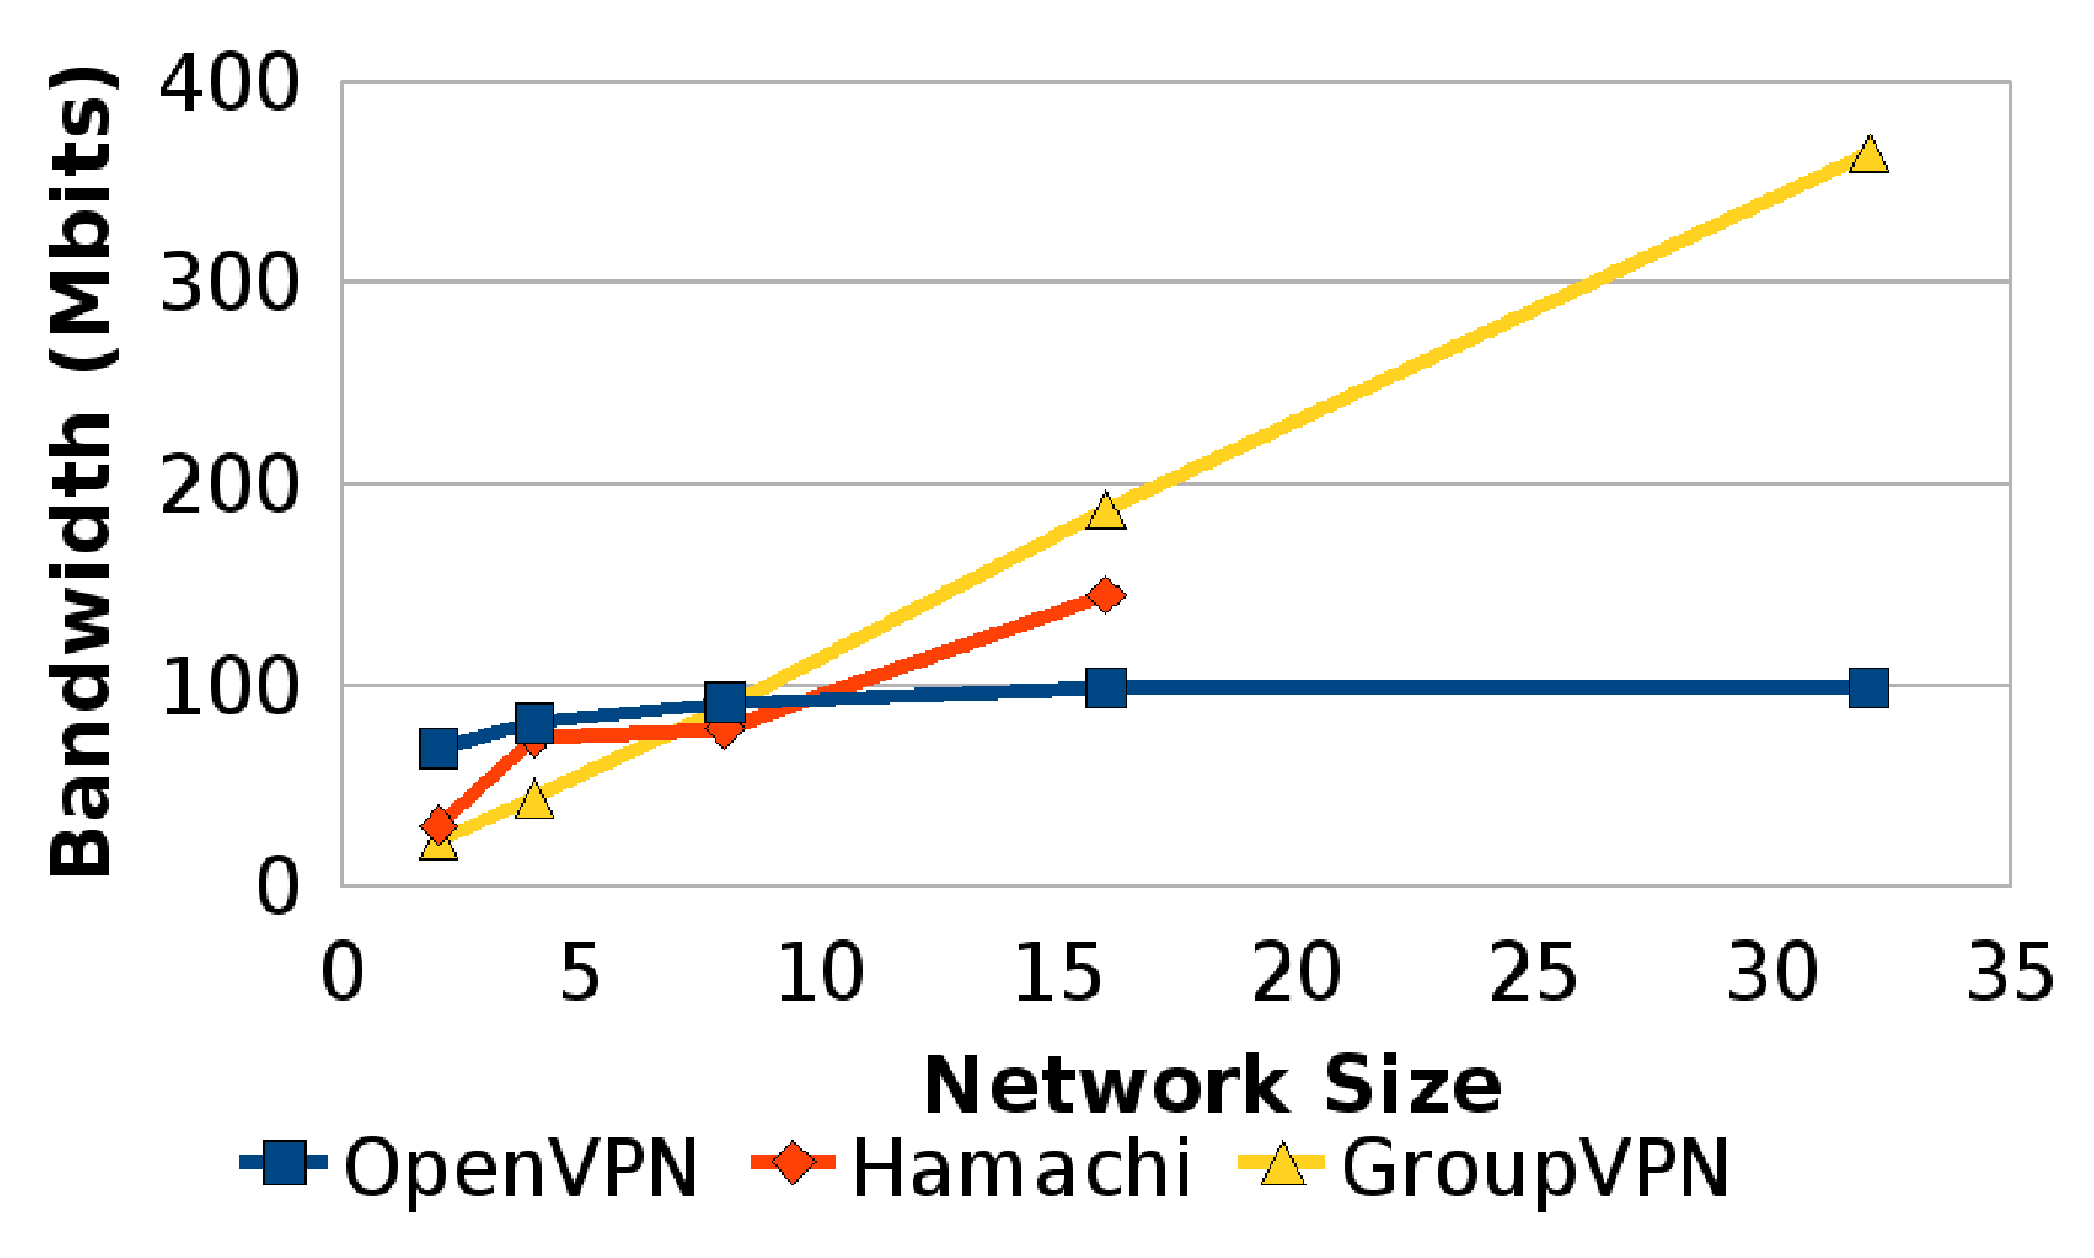
\epsfig{file=figs/bandwidth.eps, width=3in}
\caption{System bandwidth for various VPN approaches.}
\label{fig:bandwidth}
\end{figure}

Figure \ref{fig:latency} and \ref{fig:bandwidth} present the results for latency
and bandwidth respectively.  Latency is measured in transactions of successful
request/reply messages.  In the latency test, it is obvious that having the
central server increases the delay between the client and server and the results
degrade more quickly as additional peers are added to the system.  In small
systems, OpenVPN shines probably due to optimized software, though as the system
grows, the system bandwidth does not.  By the time 8 peers have entered into
the system, both decentralized approaches perform better than the OpenVPN
solution.  To summarize, decentralized VPN approaches provide better
scalability, which can be immediately noticed by low latency times and, as the
system grows, available bandwidth.

\section{Conclusions}
\label{conclusions}
As a canonical resource, this paper describe all the necessary components to
design and implement decentralized VPN approach designed to facilitate ease of
use while maintaining security and scalability.  The methods in this paper
define an abstraction for the VPN component and the features required in a
structured overlay for this style of VPN.  The VPN abstraction handles local
networking components and interacts with the overlay for communication, link
creation, and peer discovery.  In addition, we presented novel ways of
configuring the VPN through a Web 2.0 envrionment and creating full tunnel
VPNs that can be used on centralized, decentralized, and P2P VPNs.

This approach has been used to construct real systems, such as the
GroupVPN~\cite{gridappliance} and a SocialVPN~\cite{cops08}.  The GroupVPN has
been used to construct a Grid Appliance that enables the creation of distributed,
decentralized, dynamic computing grids.  Over the past 2 years, we have had an
active grid deployed for computer architecture research, Archer~\cite{archer}.  
Archer currently spans four universities with 500 resources, we have had 100s of
users who connect seamlessly to these resources from home, school, hotels, etc.
Most recently, a grid at La Jolla Institute for Allergy and Immunology went live
with minimal communication with us.  Researchers at the Clemson University and
Purdue have opted for this approach over centralized VPNs as the basis of their
future distributed compute clusters and have actively tested networks of over
1000 nodes.

While this paper introduces solutions to creating a complete structured P2P based
VPN, it introduces many new interesting research problems: 1) distributed load 
balancing of full tunnel gateways, 2) understanding the long term effects of different
automatic relay selection models, 3) understanding the benefits beyond security
of using a private overlays for a VPN such as multicast.

\bibliographystyle{IEEEtran}
\small{
\bibliography{GroupVPN}
\suppressfloats
}

\end{document}
